\documentclass{Styles/llncs}
%\documentclass[12pt,letterpaper]{article}
\usepackage{times}

\usepackage[utf8]{inputenc}
\usepackage[T1]{fontenc}

\usepackage{url}
\usepackage{graphicx}
\usepackage{caption}
\usepackage{subcaption}
\usepackage{subfig}
\usepackage{wrapfig}
\usepackage{multirow}
\usepackage{boxedminipage}
\usepackage{xspace}
\usepackage{listings}
\usepackage{listingsutf8}
\usepackage{verbatim}
\usepackage{parcolumns}
\usepackage{color}
\usepackage[usenames,dvipsnames,svgnames,table]{xcolor}
%Prevents floating item to "jump" between sections
\usepackage[section]{placeins}
\usepackage{booktabs}
\usepackage{tkz-graph}
\newcommand{\arevoir}[1]{#1}

\newcommand{\kaapi}{\textsc{\mbox{kaapi}}\xspace}

\newcommand{\libXKOMP}{\textsc{libKOMP}\xspace}

\usepackage{xcolor}
\usepackage{todonotes}
\usepackage[color,leftbars]{changebar}

\newcommand{\cfsect}[1]{(\textit{cf.} section~\ref{#1})}
\newcommand{\cfsectpage}[1]{(\textit{cf.} section~\ref{#1}, page~\pageref{#1})}
\providecommand{\figureref}[1]{\figname~\ref{#1}}
\providecommand{\cftab}[1]{(\textit{cf.} tableau~\ref{#1})}
\newcommand{\cmd}[1]{{\upshape\texttt{\symbol{"5C}#1}}}

\newenvironment{remarque}
{\description \item[Remarque:] \ \slshape}
{\enddescription}

\makeatletter
\newbox\sf@box
\newenvironment{SubFloat}[2][]%
  {\def\sf@one{#1}%
   \def\sf@two{#2}%
   \setbox\sf@box\hbox
     \bgroup}%
  { \egroup
   \ifx\@empty\sf@two\@empty\relax
     \def\sf@two{\@empty}
   \fi
   \ifx\@empty\sf@one\@empty\relax
     \subfloat[\sf@two]{\box\sf@box}%
   \else
     \subfloat[\sf@one][\sf@two]{\box\sf@box}%
   \fi}
\makeatother
\renewcommand\floatpagefraction{.9}
\renewcommand\topfraction{.9}
\renewcommand\bottomfraction{.9}
\renewcommand\textfraction{.1}
\setcounter{totalnumber}{50}
\setcounter{topnumber}{50}
\setcounter{bottomnumber}{50}
\renewcommand{\ttdefault}{pcr}
\lstset{
	tabsize=4,
%	frame=single,
	breaklines=true,
	basicstyle=\ttfamily,
	frame=tb,
	framerule=0.2pt,
%	frameround={tttt},
	showstringspaces=false,
	language=c,
%	linewidth=0.95\textwidth,
	keywordstyle=\color{black}\bfseries,
%	keywordstyle=\color{blue},
	commentstyle=\color{OliveGreen},
	stringstyle=\color{red}\itshape,
	inputencoding=utf8/latin1,
	numbers=left,
	numberstyle=\tiny,
	numbersep=5pt,
% OMP define
emph={\#,pragma, taskwait, omp, task, depend}, emphstyle=\color{RoyalBlue}\bfseries,
emph={[2]in,inout,out,cw}, emphstyle={[2]\color{BrickRed}\bfseries},
emph={[3]tied,untied,shared}, emphstyle={[3]\color{Gray}\bfseries},
emph={[4]lu0,fwd,bdiv,bmod}, emphstyle={[4]\color{DarkGreen}\bfseries},
emph={[5]cw}, emphstyle={[5]\color{DarkViolet}\bfseries},
    %moredelim=**[is][\only<3>{\color{red}}]{@}{@},
}
\lstdefinestyle{smaller}{basicstyle=\scriptsize\ttfamily}
\lstMakeShortInline|

\newcommand{\benchs}{KASTORS }

\sloppy

\begin{document}

\title{Using data dependencies to improve task based scheduling strategies on NUMA architectures}
\author{
  Philippe Virouleau$^1$ \and François Broquedis$^2$ \and Thierry Gautier$^{1,3}$
 \vspace*{-1ex}}
\institute{
   $^1$INRIA, $^2$Grenoble Institure of Technology, $^3$LIP\\
   CORSE and AVALON Teams, Computer Science Laboratories of Grenoble
   and Lyon, France\\
   \email{philippe.virouleau@inria.fr}\\
   \email{francois.broquedis@imag.fr}\\
   \email{thierry.gautier@inrialpes.fr}\\
}
\date{}
\maketitle

\begin{abstract}
  \vspace*{-5ex} The OpenMP 4.0 specifications extended the task parallelism
  constructs by providing the user a more flexible way to synchronize tasks :
  data dependencies between tasks.
  Using such an approach allows both the compiler and the runtime system
  to know exactly which data are read or written by a given task, and how these
  data will be used through the program lifetime.  Data placement and scheduling
  strategies have a significant impact on performances when considering
  NUMA architectures.  Numerous papers focus on these topics, however none
  has made extensive use of the information available through dependencies.
  One can use these information to modify the behaviour of the application at
  several levels : during initialization to control data placement,
  and during the application runtime to dynamically control both the preferred
  task placement and stealing strategy, depending on the topology.
  This paper introduces several heuristics for these strategies and their
  implementations in our OpenMP runtime XKaapi.
  We also evaluate their performances by using several linear algebra
  applications, executed on a 192 cores NUMA machine. We finally
  compare them to strategies presented previously by related works.

\smallskip
  \noindent\textbf{Keywords:}
  \emph{
    OpenMP, task dependencies, benchmark, runtime systems, NUMA, Kaapi, scheduling, workstealing
  }
\end{abstract}


\section{Introduction}

Very large non-uniform memory access (NUMA) architectures are still heavily used
nowodays, and not yet fully exploited to the best of their performances.
On such architectures the memory is distributed among several nodes, and
both bandwidth and latency depends on which processor want to access specific data,
meaning that executing each part of an application near its data is one of the key to achieve good
performances.
The recent addition of data dependencies to the OpenMP tasking model enable the
runtime to have very precise informations about which part of an application
needs which data.
This paper aims at using both these informations and the topology of the architecture
to improve data locality and task placement, to achieve better performances.

In the following sections we will first give some background about NUMA architectures
and the task programming model with data dependencies, in section \ref{sec:background}.
We will then describe our ideas and strategies to improve the runtime performances
for these applications in section \ref{sec:contributions},
as well as how we implemented them in our software. Then we will present the performances
evaluation in section \ref{sec:performances-evaluation}, where we will discuss
the results and how they behave with regard to previously suggested strategies.
We will finally present some related works in section \ref{sec:related-work}
before concluding.

TODO

task dependencies enable full knowledge about data

Different approaches for dealing with NUMA :

Initial data distribution/placement (set affinity)

Initial task placement (pushinit)

Dynamic ready-task placement (push)

Work-stealing strategies (select)

Contribution : new heuristic for these approaches, evaluation and comparison against previous one on a large NUMA machine.



%HPC architectures evolved so rapidly that it is now common to build
%shared-memory configurations with several dozens of cores.  The recent
%appearance of technologies such as the Intel Xeon Phi co-processor makes
%affordable configurations with thousands of cores a not-so-far
%reality.  Efficiently programming such large-scale platforms requires
%to express more and more fine-grain parallelism.

%Standard parallel programming environments such as OpenMP have evolved
%to address this requirement, introducing new ways of designing highly
%parallel programs. Extending OpenMP to support task parallelism stands
%as a first step to improve the scalability of OpenMP applications on
%large-scale platforms. Indeed, task parallelism usually comes with lower
%runtime-related overhead than thread-based approaches, allowing OpenMP
%programmers to create a large amount of tasks at low cost. Task
%parallelism also promotes the runtime system to a central role, as
%having more units of work to execute requires smarter scheduling
%decisions and load balancing capabilities.

%OpenMP was recently extended to support task dependencies. Instead of
%explicitly synchronizing all the tasks of a parallel region at once, the
%application programmer can now specify a list of variables a task will
%read as input or write as output instead. This information is
%transmitted to the task scheduling runtime system. The runtime then marks
%a task as ready for execution only once all its dependencies have been
%resolved. Dependencies therefore provide a way to define finer
%synchronizations between tasks, able to scale better than global
%synchronizations on large-scale platforms. Dependencies also give the
%runtime system more options to efficiently schedule tasks, as these
%become ready for execution as soon as the data they access has been
%updated.

%As promising as it looks however, any new feature needs proper
%evaluation to encourage application programmers to embrace it. While
%several compilers and runtime systems are now beginning to support
%OpenMP~4.0 task dependencies, no benchmark suite currently exists to
%evaluate their respective benefits and compare them to traditional task
%parallelism.

%This paper highlights two major contributions. We first introduce a
%new benchmark suite to experiment with OpenMP~4.0 task dependencies. We
%present performance results for both the GCC/libGOMP and the
%CLANG\footnote{Intel branch with support for OpenMP:
%\url{http://clang-omp.github.io/}}/libIOMP compilers and their runtime
%systems, comparing kernels
%involving either dependent or independent tasks. Secondly, we
%comment on the issues we met while implementing these benchmarks along
%the lines of current 4.0 revision of the OpenMP specification. Building
%on this experience, we contribute some extension proposals to the
%existing OpenMP specification, to improve the expressiveness of the
%task dependency support.

%The remainder of this paper is organized as follows. Section
%\ref{sec:omp-deps} describes the task dependency programming model in
%OpenMP~4.0. It then analyzes the strategies adopted by GCC/libGOMP and
%CLANG/libIOMP to implement this model. Section \ref{sec:benchs}
%introduces the \benchs benchmark suite we have designed to evaluate
%OpenMP~4.0's task model implementations. Section \ref{sec:perfs}
%presents the performance results of \benchs using two different hardware
%configurations. We identify and discuss practical issues with the
%current OpenMP specification, and we propose extensions in section
%\ref{sec:extensions} to address these issues. We finally present some
%related works in section \ref{sec:related-work} before concluding.

\section{Background}
\label{sec:background}
\subsection{Hardware background}
\label{sec:hardware}
Most of nowadays parallel shared memory architectures are built according to a NUMA~\footnote{Non-Uniform Memory Access} design where the memory is physically split in several banks attached to processors.
Many vendors assemble these banks in a hierarchical way, thus building shared memory machines embedding several hundreds of cores.
Exploiting such architectures at their full potential requires a fine control of the execution of a parallel application, as accessing local memory is most of the time faster than accessing memory stored in a memory bank attached to a remote processor.

The machine we experimented on is a SGI UV2000 platform made of 24 NUMA nodes.
Each NUMA node holds a 8-core Intel Xeon E5-4640 CPU for a total of 192 cores.
We refer to this machine as Intel192 in the paper. 

\begin{figure}
\begin{center}
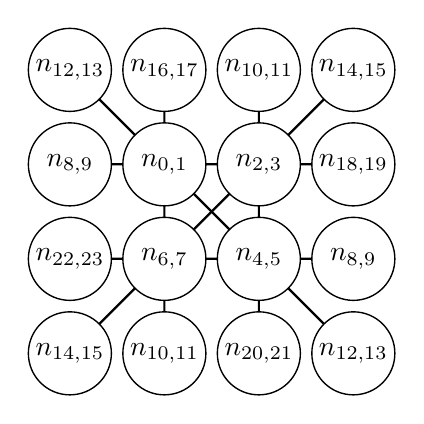
\begin{tikzpicture}[scale=0.6]
\tikzset{VertexStyle/.append style = {minimum size = 30pt, inner sep = 0pt}}

\Vertex[x=0, y=0, L=$n_{14,15}$]{n0}
\Vertex[x=0, y=2, L=$n_{22,23}$]{n4}
\Vertex[x=0, y=4, L=$n_{8,9}$]{n8}
\Vertex[x=0, y=6, L=$n_{12,13}$]{n12}
\Vertex[x=2, y=0, L=$n_{10,11}$]{n1}
\Vertex[x=2, y=2, L=$n_{6,7}$]{n5}
\Vertex[x=2, y=4, L=$n_{0,1}$]{n9}
\Vertex[x=2, y=6, L=$n_{16,17}$]{n13}

\Vertex[x=4, y=0, L=$n_{20,21}$]{n2}
\Vertex[x=4, y=2, L=$n_{4,5}$]{n6}
\Vertex[x=4, y=4, L=$n_{2,3}$]{n10}
\Vertex[x=4, y=6, L=$n_{10,11}$]{n14}
\Vertex[x=6, y=0, L=$n_{12,13}$]{n3}
\Vertex[x=6, y=2, L=$n_{8,9}$]{n7}
\Vertex[x=6, y=4, L=$n_{18,19}$]{n11}
\Vertex[x=6, y=6, L=$n_{14,15}$]{n15}

\Edge(n0)(n5)
\Edge(n4)(n5)
\Edge(n1)(n5)

\Edge(n13)(n9)
\Edge(n12)(n9)
\Edge(n8)(n9)

\Edge(n15)(n10)
\Edge(n14)(n10)
\Edge(n11)(n10)

\Edge(n3)(n6)
\Edge(n2)(n6)
\Edge(n7)(n6)

\Edge(n9)(n5)
\Edge(n9)(n10)
\Edge(n5)(n10)
\Edge(n9)(n6)
\Edge(n5)(n6)
\Edge(n10)(n6)

\end{tikzpicture}
\end{center}
\caption{Memory topology of the Intel192 SGI UV2000 machine.}
\label{fig:idchire}
\end{figure}

Figure \ref{fig:idchire} shows the Intel192 machine memory topology.
NUMA nodes are organized by pairs of nodes connected together through Intel QuickPath Interconnect.
These pairs can communicate together through a proprietary fabric called NUMALink6, represented by the edges on the graph.
In other words, taking node $n_0$ as example :
\begin{itemize}
\item node $n_0$ communicates with node $n_1$ through Intel QPI ;
\item node $n_0$ is one hop away from node $n_4$ \emph{(e.g. communications between node $n_0$ et node $n_4$ cross one NUMALink6 memory controller)};
\item node $n_0$ is two hops away from node $n_{20}$ \emph{(e.g. communications between node $n_0$ et node $n_{20}$ cross two NUMALink6 memory controllers)};
\end{itemize}

Table \ref{tab:idchire} shows the distances advertised by the hwloc library~\cite{DBLP:conf/pdp/BroquedisCMFGMTN10} that represent factors on the communication time, communicating from node $n_0$ to any other node of the Intel192 machine, whether the node is a peer (node $n_1$ in this case), is located one hop away (nodes $n_2$ to $n_9$, $n_{12}$, $n_{13}$, $n_{16}$ and $n_{17}$) or is located two hops away (nodes $n_{10}$, $n_{11}$, $n_{14}$, $n_{15}$ and $n_{18}$ to $n_{23}$). These factors, which have been correlated with experimental values on both bandwidth and latency by Pilla et al.~\cite{pilla:tel-00981136}, show how much impact the architecture topology may have on a parallel application performance.

\vspace{-0.5cm}

\newcolumntype{C}[1]{>{\centering\let\newline\\\arraybackslash\hspace{0pt}}m{#1}}

\begin{table}
\caption{NUMA distances from node 0 advertised by the hwloc library on Intel192.}
\begin{center}
\begin{tabular}{C{3cm} C{2cm} C{2cm} C{2cm} C{2cm}}
    \toprule[0.15em]
		\emph{NUMA nodes location} & \emph{local} & \emph{peer} & \emph{one hop away} & \emph{two hops away} \\
    \midrule[0.1em]
	hwloc distances & 1.0 & 5.0 & 6.5 & 7.9 \\
    \bottomrule[0.15em]
\end{tabular}
\end{center}
\label{tab:idchire}
\end{table}

\vspace{-1cm}

\subsection{Software background}

To exploit such large-scale shared memory architectures, the application programmer needs :
\begin{enumerate}
\item to express massive fine grain parallelism to get the most out of the numerous processing units of the platform ;
\item to control the execution of the application, especially the way computations and data are distributed over the platform, to prevent the NUMA design to have a negative impact on the overall application performance.
\end{enumerate}

Task-based parallel programming environments provide ways of expressing fine grain parallelism that can be dynamically assigned to processors at runtime.
OpenMP~\cite{openmp40}, the de-facto standard for shared-memory parallel programming, supports task parallelism with dependencies since revision 4.0.

\subsubsection{A glimpse at OpenMP tasking}

An OpenMP \emph{task} can be seen as an independant \emph{unit of work} an OpenMP thread can execute.
Tasks can be created by an OpenMP thread and executed by any thread of the same parallel region. 
As managing tasks at runtime is way cheaper than creating and synchronizing threads, the application programmer can take the parallelization of its application further, as he can now consider portions of code that were too fine grain to be parallelized using only threads.
The synchronization of OpenMP 3.0 tasks is performed thanks to the |taskwait| keyword that waits for the completion of all the tasks generated from the current OpenMP parallel region.
On one hand, the application programmer is responsible for creating and synchronizing OpenMP tasks explicitly. 
On the other hand, the runtime system is in charge of assigning tasks to threads during the application execution, considering the underlying system state.

OpenMP 4.0 pushes the concept of task further introducing the |depend| keyword to specify the access mode of each shared variable a task will access during its execution. 
Access modes can be set to either |in|, |out| or |inout| whether the corresponding variable is respectively read as input, written as output or both read and written by the considered task. 
This information is then processed by the underlying runtime system to decide whether a task is ready for execution or should first wait for the completion of other ones.

Listing 1.1 shows the implementation of a blocked matrix multiplication. It is
taken from the official OpenMP 4.0 examples~\footnote{available at http://www.openmp.org}.
Running this |depend| version of the program leads to the creation of a dependency graph.
A task created on line 7 can thus be executed \emph{as soon as} the data they access has been updated by its predecessors in this graph.
When an OpenMP thread turns idle, the runtime system browses this graph to decide which task should be executed next, according to tasks' current state and resolved dependencies.

Task dependency support comes with several benefits. 
First, task dependencies involve decentralized, selective synchronization operations that should scale better than the broad-range taskwait-based approaches.
In some situations, this way of programming unlocks more valid execution scenarios than explicitly synchronized tasks, which provides the runtime system with many more valid task schedules to choose from. 
As an added benefit, information about task dependencies also enables the runtime system to optimize further, such as improving task and data placement on NUMA systems, like detailed in this paper.

\vspace{-0.5cm}

\begin{figure}[htbp]
\begin{lstlisting}[caption=Blocked matrix multiplication with OpenMP task dependencies,frame=tlrb,style=smaller,label=lst:MM-deps]{lst:MM-deps}
// Assume BS divides N perfectly
void matmul_depend(int N, int BS, float A[N][N], float B[N][N], float C[N][N]) {
     int i, j, k, ii, jj, kk;
     for (i = 0; i < N; i+=BS) {
          for (j = 0; j < N; j+=BS) {
               for (k = 0; k < N; k+=BS) {
                    #pragma omp task depend (in: A[i:BS][k:BS], B[k:BS][j:BS]) \
                         depend (inout: C[i:BS][j:BS])
                    for (ii = i; ii < i+BS; ii++)
                         for (jj = j; jj < j+BS; jj++)
                              for (kk = k; kk < k+BS; kk++)
                                   C[ii][jj] = C[ii][jj] + A[ii][kk] * B[kk][jj];
               }
          }
     }
}
\end{lstlisting}
\end{figure}

\vspace{-1cm}

\subsubsection{The way we execute task-based applications}

Most task-based programming environments rely on a work-stealing execution model, originally introduced in Cilk~\cite{cilk5}. 
Work-stealing is indeed often considered when it comes to dynamically balance the work load among processing units. 
The work-stealing principle can be summarized as follows. 
An idle thread, called a thief, initiates a steal request to a randomly selected victim. 
On reply, the thief receives a copy of one ready task, leaving the original task marked as stolen.
Coherency between a thief and its victim is ensured by a variant of Cilk's T.H.E protocol, also described in \cite{cilk5}.

The runtime system we develop, called \kaapi, also implements the work-stealing execution model to execute OpenMP task-based applications.
The runtime creates a system thread, called a \emph{kproc}, for each processing unit to be used.
On a NUMA multicore machine, a processing unit is a core.
A kproc creates tasks and pushes them on its own work queue, which is implemented as a stack.
The enqueue operation is very fast : it takes around ten cycles on modern x86/64 processors~\cite{libkomp}.
As in Cilk, a  running \kaapi task can create children tasks. 
During the execution of a task-based application, if a kproc encounters a task that is marked as stolen, it suspends its execution and switches to
the work stealing scheduler that waits for dependencies to be met before
resuming the kproc execution. 

To find a ready task, a thief kproc iterates through the victim's queue from
the least recently pushed task to the most recently one and it computes true
data-flow dependencies for each task. 
%False dependencies are resolved through variables renaming. 
The iteration stops as soon as the kproc finds a ready task on the victim's queue.

In addition, \kaapi promotes a cooperative way of stealing tasks,
enabling multiple steal requests to the same processor to be served at once~\cite{DBLP:conf/europar/TchiboukdjianDGMR10}.
In practice, if the victim kproc is in a stealing state, the thief aborts the steal request and selects another victim randomly.
The \kaapi cooperative stealing algorithm divides the work into $k+1$ pieces when $k$ steal requests target the same processor.

\subsection{Summary}
Task-based programming environments stand as a promising candidate to exploit large-scale NUMA machines.
They give the application programmer the ability to generate the massive fine-grain parallelism that is desperately needed to occupy every processing unit of such architectures.
The work-stealing execution model they rely on also fill the need for balancing the application workload in a dynamic way, both tackling applications with irregular workloads and improving the overlapping of non-uniform memory access with actual computation.
However, exploiting NUMA architectures at their full potential requires some control on the way tasks and data are distributed over the platform, in order to avoid NUMA-related performance penalties. 
Preserving data locality while guaranteeing dynamic load balancing at runtime imposes an embarrassing dilemma to the runtime system that has a direct impact on :
\begin{itemize}   
\item the way data are allocated ;
\item the way ready tasks are originally assigned to processors ;
\item the way the scheduler browses the architecture topology to find a processor to steal tasks from.
\end{itemize}

The following of the paper study all these aspects and how they impact on each other, and more generally how they affect the overall application performance.

\section{Using OpenMP tasks dependencies to improve tasks and data
  placement on NUMA machines}
\label{sec:contributions}

In this section, we describe how the runtime system can have a positive impact on the application execution using the information provided by data dependencies.
The following sections describe the way we adapted the behavior of the runtime system to control data placement during the initialization phase, when data will be allocated and accessed for the first time, and how we modified the way tasks that perform the actual computations are dynamically assigned to processors while maximizing data locality.


\subsection{Inside the \kaapi task-based runtime system}

This section describes some of the key internal structures and mecanisms of the \kaapi runtime system.

\subsubsection{The way \kaapi models the architecture}

\begin{figure}[t]
  \centering
  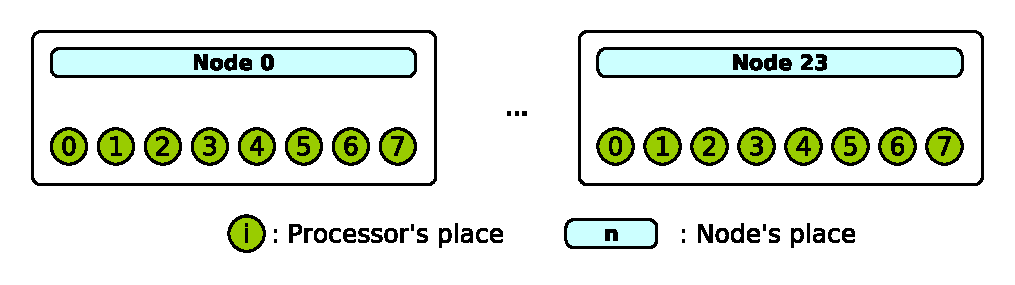
\includegraphics[scale=0.5]{./figures/topology.pdf}
\caption{Processors and Nodes representation}
\label{fig:detail-topology}
\end{figure}

\kaapi sees the architecture topology as a hierarchy of \verb/places/.
A \verb/place/ is a list of tasks associated to a subset of the machine processing units.
\kaapi's places are very similar to the notion of \emph{shepherd} introduced in \cite{DBLP:journals/ijhpca/OlivierPWSP12}, or ForestGOMP's \emph{runqueues}~\cite{BroFurGogWacNam10IJPP}.
\kaapi most of the time only considers two levels of places : node-level places, which are bound to the set of processors contained in a NUMA node, and processor-level places, which are bound to a single processor of the platform.
This way, at the processor level one \verb/place/ is associated to each of the physical cores, and
at the NUMA node level one \verb/place/ is associated to each of the NUMA nodes, like represented in
Figure \ref{fig:detail-topology}.


\subsubsection{The way \kaapi enables ready tasks and steal them}

When a processor becomes idle, the runtime system browses the topology to find a place from which stealing a task.
There are many ways to do so, implemented in different \emph{selection strategies} called \verb/WSselect/, for \emph{work-stealing select} in the remaining of the paper.
Once a place is selected, the processor will take a ready task from its queue.

The completion of a task most of the time unlocks the execution of some of its children in the dependency graph.
This means marking them as ready for execution and pushing at least one of them to a place.
Once again, there are many ways of selecting the place where to push ready tasks, implemented in strategies we refer to as \verb/WSpush/, for \emph{work-stealing push}.

\subsection{Controlling data distribution on a NUMA system}
Controlling the way data are allocated on a NUMA system requires a good understanding of the underlying memory architecture.
Application programmers can achieve this using dedicated tools or libraries, like libNUMA's \verb!numactl!~\cite{DBLP:journals/corr/abs-1101-0093}, which can be used to set a default memory allocation policy for the whole application.
For example, the \verb!--interleave=all! memory policy spreads out all the memory pages of dynamically allocated variables over all the NUMA nodes of the machine.
This policy is widely used on NUMA systems in conjonction with dynamic parallelism, like task-based programs, as it distributes the memory traffic over all the memory controllers, making processors "\emph{all equally bad}" when it comes to access memory.
To better control data placement, parallel application programmers are used to rely on the \emph{first-touch} allocation policy, which is the default behavior for memory allocation on most Linux systems.
This allows to allocate memory pages when they are accessed for the first time.
Using this policy, a memory page is allocated on the same NUMA node than the first thread that accesses it.
Many parallel applications perform the initialization of data structures in parallel, to indirectly distribute data thanks to the first-touch policy.
However, in order to avoid remote memory accesses, the threads must access the data during the computation phase the exact same way it was accessed during the initialization phase, which is very difficult to guarantee with dynamic task-based parallelism.

To better control data distribution on NUMA systems, we propose two different approaches :
\begin{itemize}
\item either the application programmer explicitly allocates data on specific NUMA nodes of the machine through a dedicated API we provide (\verb!omp_set_affinity)!;
\item or the application programmer only marks some regions of code that initialize data to give the runtime system the opportunity to map the corresponding tasks to make the first-touch allocation policy indirectly apply the data distribution we target. Indeed, Olivier et al.~\cite{Olivier:2012:CMW:2388996.2389085}
have shown that specifying affinity for initialization tasks can lead to huge improvement over locality oblivious techniques.
\end{itemize}
Both of these approaches give the runtime system a way of keeping track of where the memory pages associated to the application data are actually stored.
This information is then used to guide the way we perform task creation and load balancing.

We have implemented three data distribution strategies : \verb!cyclicnuma! which distributes the data in a round-robin fashion over the NUMA nodes ; \verb!randnuma! which randomly distributes the data over the NUMA nodes and \verb!defaultnuma! which distributes the data according to the affinity hints provided by the application programmer using \verb!omp_set_affinity!.
Note that unlike \verb!numactl!, the strategies we implemented consider the whole data appearing in the OpenMP task \verb!depend! clause instead of working at the page level. In other words, while the two memory pages holding a 8K-long array would be distributed on different nodes by \verb!numactl --interleave=all!, they are always assigned to the same NUMA node when using one of our data distribution strategies.

\subsection{Distribution of ready tasks : WSpush strategies}

This section describes four different ways of pushing ready tasks to a NUMA system places.
Two of them are data-oblivious, while the other two rely on the dependencies expressed using the \verb!depend! keyword on OpenMP tasks.

The \verb/pLoc/ strategy makes a processor push ready tasks to
    its own place, while the \verb/pLocNum/ strategy makes a processor push ready tasks to the place of its NUMA node (\emph{local NUMA node}).
The \verb/pNumW/ strategy pushes tasks on the node-level place corresponding to the NUMA node where most of their output data are allocated on (W stands for Write).
The last WSpush strategy, called \verb/pNumWLoc/, behaves almost the same than \verb!pNumW! except that if
    the data are allocated on the NUMA node of the processor pushing the task, we directly push the task to this processor's place instead of pushing it to the node-level place (Loc stands for Local).
    
    It's important to note that \verb!pLoc! and \verb!pLocNum! does not take initial data placement into account, while \verb!pNumW! and \verb!pNumWLoc! are both aware of where a task's data are physically allocated and which of them are written, thanks to the OpenMP \verb!depend! keyword.

\subsection{Dynamic load balancing using work-stealing : WSselect strategies}

Another important step when implementing work-stealing is the selection of the victim processor we want to steal from.
This section describe the selection strategies we implemented, that take the architecture memory hierarchy into account.

The first two strategies, \verb!sRand! and \verb!sRandNum! are similar to those studied in~\cite{DBLP:journals/ijhpca/OlivierPWSP12}
and distinguish two levels of hierarchy : the processor level and the NUMA node level.
\verb/sRand/ selects a random processor's place while \verb/sRandNum/ selects a random NUMA node's place.

We additionally implemented several strategies mixing both levels of hierarchy,
described below.

\begin{figure}[t]
  \centering
  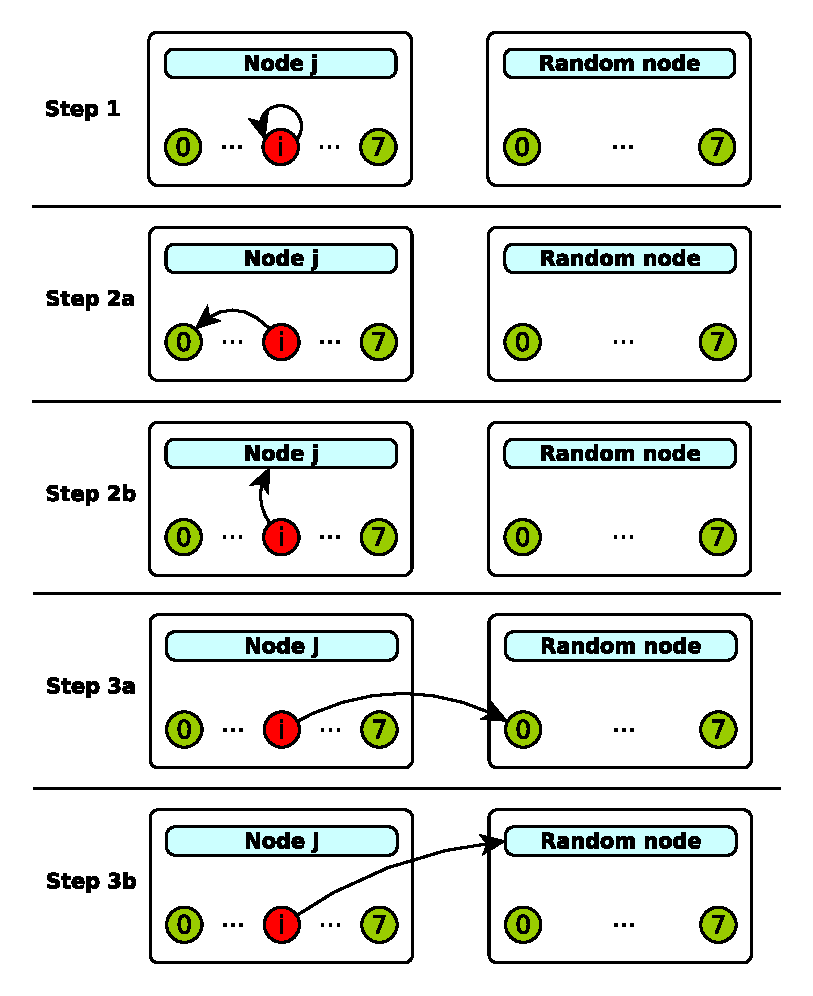
\includegraphics[scale=0.7]{figures/strategies.pdf}
\caption{Illustration of the "sProcNum" strategy}
\label{fig:detail-strategy}
\end{figure}
\begin{itemize}
  \item \verb/sProcNum/ : this strategy is illustrated in figure \ref{fig:detail-strategy}.
    First, we browse the processor's place (1). Upon failure, we browse the topology in the following order : we first browse one of the neighbor processors (2a); when all the neighbors have been visited, we browse the local NUMA place (2b); we continue by browsing all the processors' places from a random remote node (3a) and we eventually consider the place of its NUMA node (3b).
  \item \verb/sNumProc/ : This strategy is similar, except we always look at the
    NUMA place before looking at the processors' place (in figure \ref{fig:detail-strategy}
    it means we switch step 2a with 2b, and step 3a with 3b).
  \item \verb/sProc/ : In this strategy the stealer will visit only the
    processors' places and its own NUMA place. In figure \ref{fig:detail-strategy} it means we do
    every steps but step 3b.
  \item \verb/sNum/ : In this strategy the stealer will visit only NUMA places
    and its neighbour. In figure \ref{fig:detail-strategy} it means we do
    every steps but step 3a.
\end{itemize}

Like proposed in \cite{Olivier:2012:CMW:2388996.2389085}, all these strategies come in two versions : a \verb!strict! version in which we prevent processors from stealing from other NUMA nodes to improve data locality, and a \verb!loose! version where these restrictions do not apply.
For example, the \verb!strict! version of the \verb!sProcNum! strategy could be illustrated by the same kind of diagram as figure \ref{fig:detail-strategy} except we would not go though steps 3a and 3b.

\section{Evaluation}
\label{sec:performances-evaluation}

\subsection{Experimental setup}

We ran all our experiments on the Intel192 machine described in section \ref{sec:hardware}.

We evaluated our strategies using the KASTORS~\cite{virouleau:hal-01081974}\footnote{git available at https://scm.gforge.inria.fr/anonscm/git/kastors/kastors.git, tag "tag-europar16"} benchmark suite.
More specifically, we used the dependent tasks version of the blocked QR factorization
(\verb/dgeqrf_taskdep/), and of the blocked Cholesky factorization (\verb/dpotrf_taskdep/).

These applications rely on kernels from BLAS and LAPACK libraries, we used OpenBLAS 2.15
to provide them.

We used the \kaapi runtime system. We tagged the version we used on \kaapi's
git repository\footnote{https://scm.gforge.inria.fr/anonscm/git/kaapi/kaapi.git } in the branch \emph{public/europar2016}.
For all of the above applications, we used the GCC 5.2.0 release compiler.

We made our execution log files public\footnote{TODO}, as well as all the scripts we used, so that
anyone may reproduce our data analysis.

\subsection{Impact of the data distribution}

We first evaluated the impact the initial data distribution has on the application performance. We did an evaluation for multiple matrix sizes and block sizes,
as well as multiple combinations of WSpush and WSselect strategies. Figure \ref{fig:eval-distrib} reports the
results we obtained for the Cholesky application, on 32K-wide matrices divided in blocks of 512$\times$512 elements. We observed similar behavior running Cholesky on different matrix sizes (16K to 64K) and block sizes (256 to 1024).

\begin{figure}[t]
  \centering
  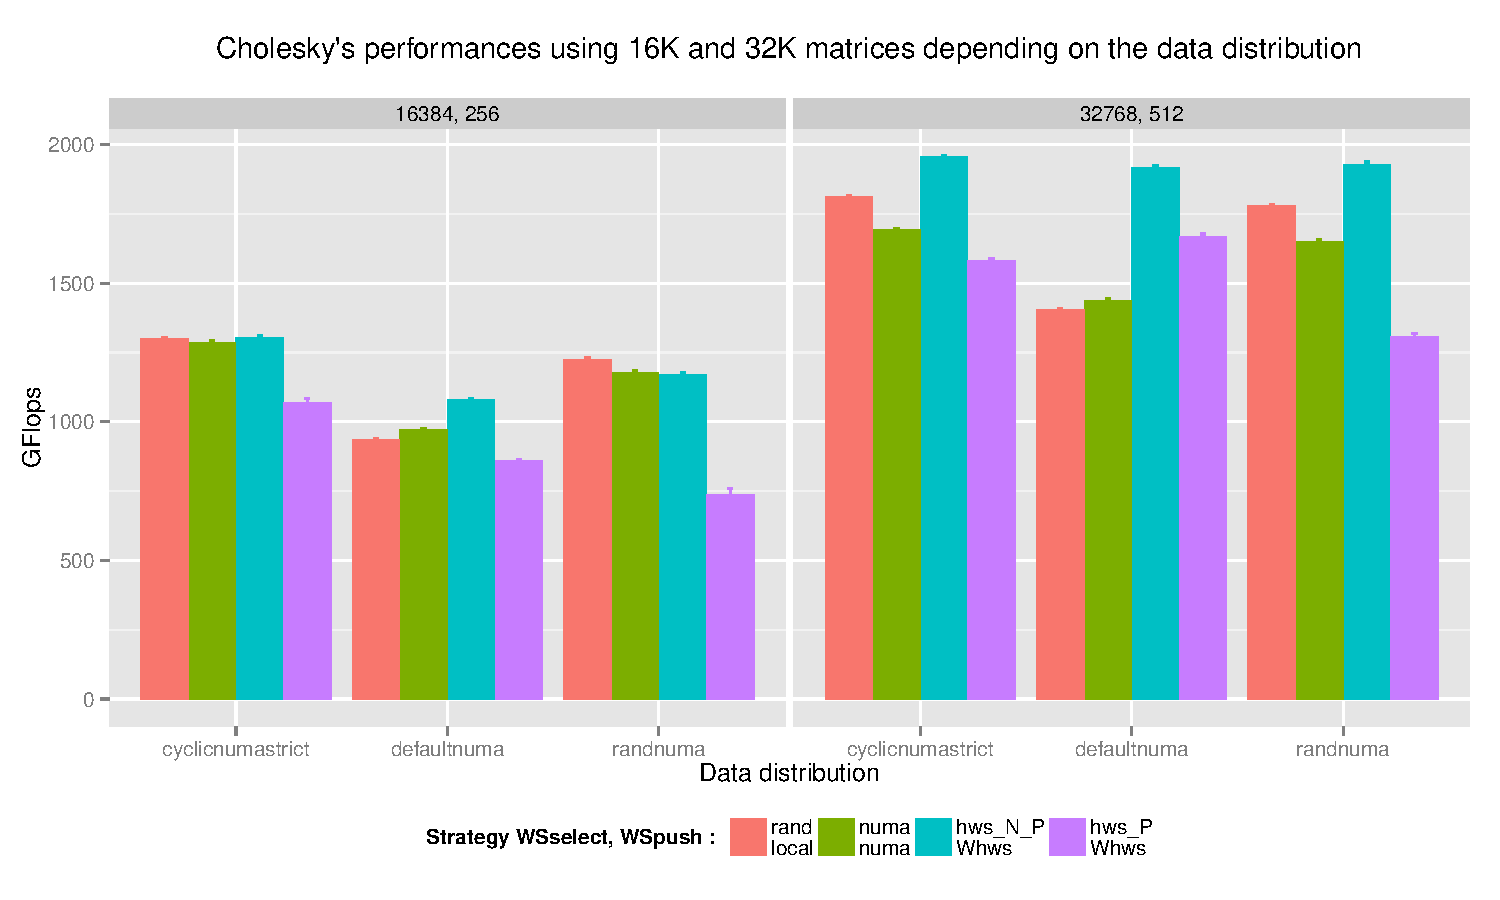
\includegraphics[scale=0.5]{figures/graph_distrib.pdf}
\caption{Evaluating several data distributions}
\label{fig:eval-distrib}
\end{figure}


TODO Conclusion : gérer la distribution c'est indispensable, après cyclicnuma a l'air suffisant.


\subsection{Impact of the stealing restriction}

Given a data distribution, previous works~\cite{Olivier:2012:CMW:2388996.2389085}
have shown that restricting the task execution to the node where the data are
written leads to better data locality which may improve the application performance.

%Note explicative :
% Pour i dans 0-N le kernel dpot agit sur chaque bloc de la diagonale
% Au rang i,
% - trsm agit sur la colonne en dessous de la case i,i
% - syrk agit sur toutes les cases de la diagonale à partir de i+1,i+1 jusqu'à n,n
% - gemm agit sur le reste des cases de la triangulaire inférieure non touchées par trsm ou syrk
% Bref : il y a 64 tiles en round robin, ça fait un peu moins de 3 tiles/noeuds, sur 64 tiles
% seulement 36 sont écrites, parmis elles la colonne inférieure 1 est écrite 1 fois,
% la 2 deux fois, etc. Chaque case i,i est écrite i+1 fois, les dépendances
% en écriture sont donc très largement concentrées sur la partie inférieure droite de la matrice !
% Donc le strict c'est nul.
However, this is heavily dependent on the algorithm the application implements. For instance, in the case
of a Cholesky factorization, many tasks write to the diagonal tiles
of the matrix comparatively to other tiles of the matrix. Therefore applying
a steal restriction on those task will potentially lead to an important number
of inactive processors.

We evaluated both strict and loose versions of our work-stealing strategies and found
out that preventing processors from stealing from other NUMA nodes can lead to a loss of performance by
around 25\% to more than 75\% with respect to the same setup without the \emph{strict}
restriction.

For the sake of brevity we did not include a figure for this, but the results of these
experiments are included in the logs publicly published.


%\begin{figure}[t]
  %\centering
  %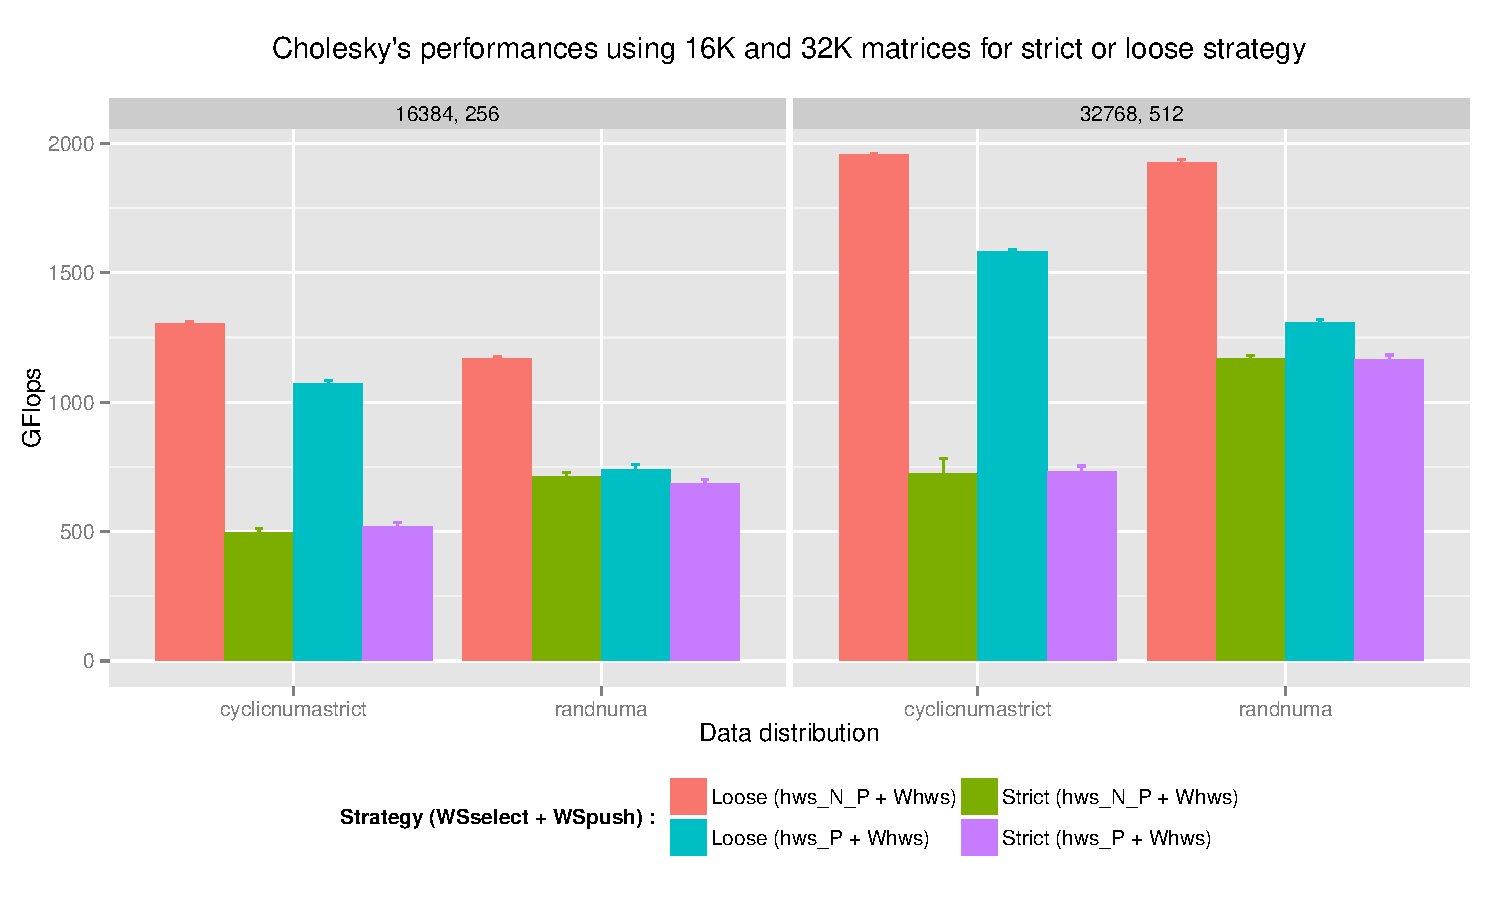
\includegraphics[scale=0.6]{figures/graph_strict.pdf}
%\caption{Evaluating impact of strictness}
%\label{fig:eval-strict}
%\end{figure}


\subsection{Overview of the strategies performances}

We took a given data distribution, \verb/cyclicnuma/, and compared the
different strategies, without any steal restriction.
Once again, even if the performances obtained where obviously not the same, the behaviour
of the different strategies comparatively to each others were similar for the
different applications.

Figure \ref{fig:eval-all-strat} shows the results of the experiments for the
Cholesky algorithm, using matrices of size 32768, with a blocksize of 512 (best configuration).


One first interesting fact to note is that even with very basic \verb/WSselect/
and \verb/WSpush/ strategies (\verb/sRand/+\verb/pLoc/), we get decent performances
thanks to the distribution.

Another remark : given a selection strategy (e.g. \verb/sRandNum/), placing
the task on the NUMA node where the written data are allocated (\verb/pNumW/) gives
better result than simply pushing the data to its NUMA node (\verb/pLocNum/).

Assuming the tasks are pushed using the \verb/pNuwWLoc/ strategy, focusing
place selection only on one level of the hierarchy (\verb/sProc/ or \verb/sNum/)
fails to reach performances we could obtain using naive strategies.

On the contrary, taking into account both level of the hierarchy (\verb/sProcNum/,
\verb/sNumProc/) achieve similar and better performances than other strategies.



\begin{figure}[t]
  \centering
  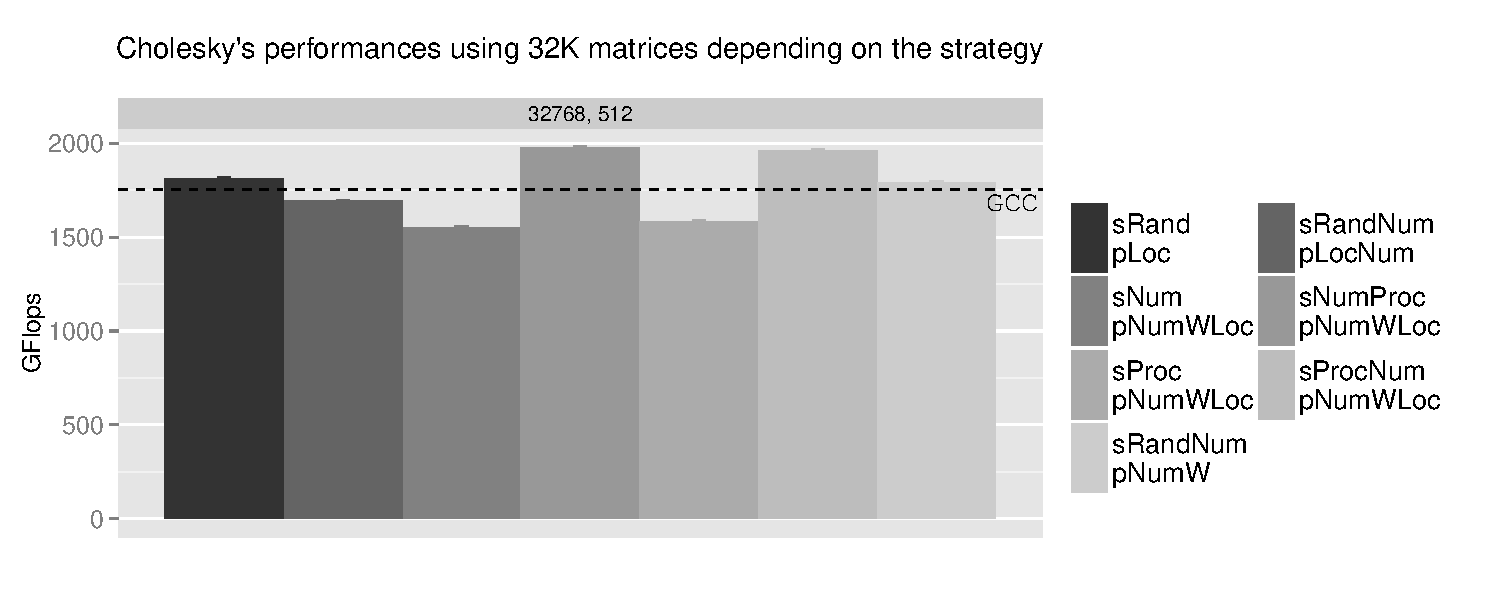
\includegraphics[scale=0.5]{figures/graph_all_strat.pdf}
\caption{Evaluating all strategies}
\label{fig:eval-all-strat}
\end{figure}


\subsection{Strategies performance scaling}

Figure \ref{fig:eval-strat-sizes} shows the behaviour of the different strategies
depending on the matrix size and block size, again using a \verb/cyclicnuma/ distribution
without steal restriction. The figure shows the performances using
the best block size for each matrix size (which is, for our setup, 256 for a matrix
size of 16384, and 512 for the others).

\begin{figure}[t]
  \centering
  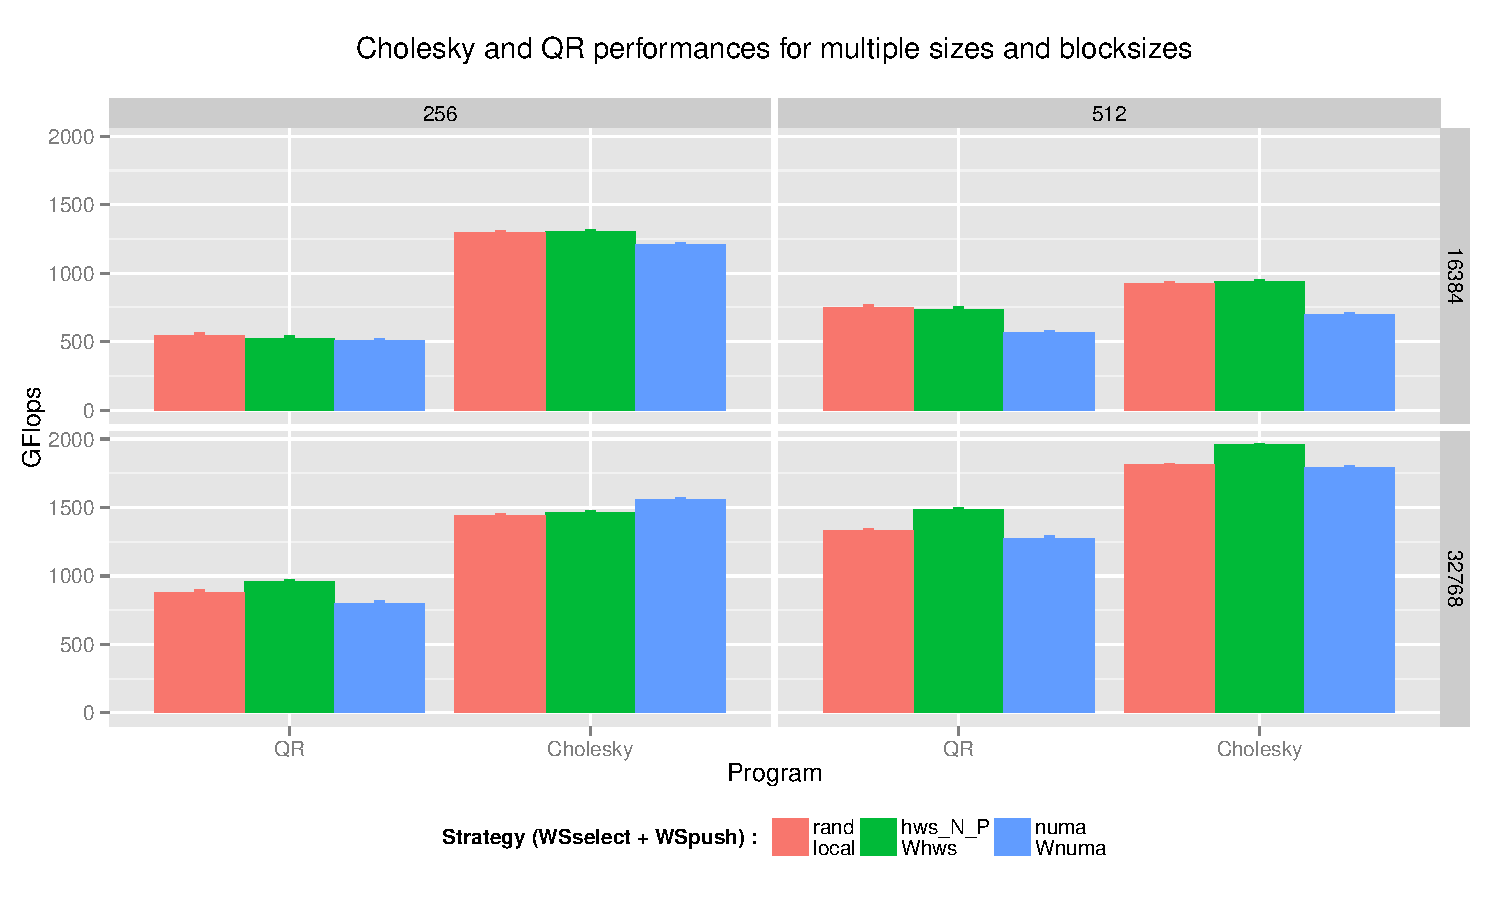
\includegraphics[scale=0.5]{figures/graph_details_strat.pdf}
\caption{Evaluating specific strategies on multiple sizes}
\label{fig:eval-strat-sizes}
\end{figure}


From the previous experiment results, we selected a subset of three strategies
combination for this evaluation :
\begin{itemize}
  \item \verb/sRand/ + \verb/pLoc/, which is a basic not hierarchy-aware strategy
  \item \verb/sNumProc/ + \verb/pNumWLoc/, which was the best strategy in our previous
    evaluation, and is also equivalent to using \verb/sProcNum/.
  \item \verb/sRandNum/ + \verb/pNumW/. Two combinations use the \verb/sRandNum/,
    the one taking into account data locality is simply better.
\end{itemize}
We chose not to select \verb/sNum/ or \verb/sLoc/, as they use the same \verb/WSpush/
as our second combination, but with relatively worse performances.

As expected, taking both hierarchy and data locality into account (\verb/sNumProc/
+ \verb/pNumWLoc/) gives overall the best performances.
The only exceptions are for small matrix sizes (16384), where there may just be
not enough work to be able to take advantage of this strategy.

We must note that simply distributing the data over the nodes enables the basic
\verb/sRand/ + \verb/pLoc/ combination to achieve satisfying performances.


\section{Related work}
\label{sec:related-work}

Numerous works focus on data locality and/or topology-aware scheduling strategies for
NUMA architectures~\cite{DBLP:conf/europar/Clet-OrtegaCP14,DBLP:journals/ijhpca/OlivierPWSP12,Olivier:2012:CMW:2388996.2389085,DBLP:journals/corr/Tahan14,DBLP:conf/europar/TerbovenSCM12,DBLP:journals/corr/abs-1101-0093}, however none takes advantage of the OpenMP \verb/depend/ clause,
which indicate precisely which data matter for a given task, and from which
the runtime can take valuable information for scheduling its tasks.

TODO parler des schedule static.

\begin{itemize}
\item Ce qu'on fait, c'est mieux que Bronis parce qu'on a la vision
  (et le contrôle indirect) du placement des données. Encore faut-il
  le démontrer! Une coucourbe hwsnumafirst.numa.* (TODO : à vérifier)
  devrait suffire à montrer que ce qu'on fait va plus loin (en termes
  de perfs) que ce qu'ils proposaient.
\item La question qui tue (Thierry ?) : si on est capable de contrôler le
  placement des tâches dans les kprocs, et de contrôler le placement
  mémoire, pourquoi on ne fait pas de placement statique à la SCOTCH
  ou autre?
\end{itemize}

CEA~\cite{DBLP:conf/europar/Clet-OrtegaCP14},
Bronis~\cite{DBLP:journals/sp/OlivierSSP13} TODO: c'est peut-être pas
la bonne ref pour Bronis, OpenMP task-scheduling et
NUMA~\cite{DBLP:journals/corr/Tahan14}, solution au niveau appli
(terboven)~\cite{DBLP:conf/europar/TerbovenSCM12}, Olivier et al.~\cite{DBLP:journals/ijhpca/OlivierPWSP12}.

\section{Conclusion and future works}

\section*{Acknowledgments}

FIXME citer ELCI !

This work has been partially supported by the IRSES2011-295217
HPC-GA Project.

  \small \bibliographystyle{Styles/iplain}
%\nocite{*}
  \bibliography{Bib/paper}

\end{document}
